\chapter{NoSQL}\label{nosql}
NoSQL is labeled as a next generation database known to most as ``Not only SQL" \cite{nosql1}. This definition however insinuates its defiance against the industry standard SQL. It was originally developed in 1998 by Carlo Strozzi; a member of the Italian Linux society, with the intention of being a non-relational, widely distributable and highly scalable database. Strozzi named the database management system NoSQL to merely state it does not express queries in the traditional SQL format. Sadalage and Fowler believe the definition we commonly refer NoSQL as comes from a 2009 conference in San Fransisco held by Johan Oskarsson, a software developer. Sadalage and Fowler recall Oskarssons desire to generate publicity surrounding the event and in an attempt to do so devised the twitter hashtag ``NoSQL Meetup". The main attendees at the conference debrief session were Cassandra, CouchDB, HBase and MongoDB and so the association stuck. \cite{nosql1}

NoSQL solutions are not bound by a definitive schema structure. This permits the ability to freely adapt database records or add custom fields for example without considering structural changes. This is extremely effective when dealing with varying data types and data sets, in comparison to the traditional relational database model which when tackling this issue often resulted in ambiguous field names.  \cite{nosql1}

\section{Brewer's CAP Theorem}\label{captheorem}


\section{Database Classification}\label{dbclass}
One of the first decisions to be made when selecting a database is the characteristics of the data you are looking to leverage. \cite{nosql2} There are a multitude of options available with many different classifications. The following sections discuss a subset of these which are relevant to this project.

\subsection{Distributed Database}\label{distributeddb}
A distributed database (DDB) comprises of two or more data files located at different sites and servers on a computer network. \cite{dd} The advantage of using a DD is that as the database is distributed, multiple users can access a portion of the database at different locations locally and remotely without obstructing one another's work. It is  pivotal for the DD database management system to periodically synchronise the scattered databases to make sure that they all have consistent data.  \cite{dd} For example if a user updates or deletes data in one location is is essential this change is mirrored on all databases. This ability to remotely access a database from all across the world lends itself to not only multinational companies for example but also startup businesses which recruit the expertise of others from various locations.

\subsection{Document-Oriented Database}
Document-orientated database (DODB) are designed for storing, retrieving and managing document files such as XML, JSON and BSON. The documents stored in a DODB model are data objects which describe the data in the document, as well as the data itself. \begin{figure}[h]\begin{center}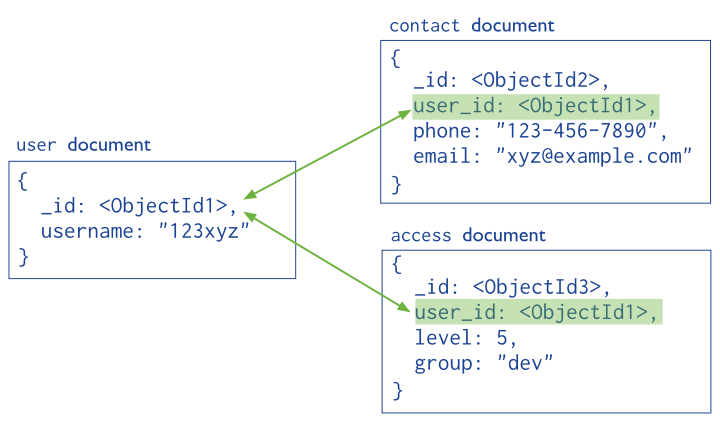
\includegraphics[width=0.75\linewidth]{images/mongodbmodel}\caption{MongoDB document}\label{fig:mongo}\end{center}\end{figure} Figure \ref{fig:mongo} illustrates an example document stored in a DODB specifically in MongoDB. The data is a recognisable JSON format and the joins of the document are between common variable values within each document.

\subsection{Graph-Orientated Database}
A graph-oriented database (GODB), is a form of NoSQL database solution that uses graph theory to store, map and query relationships. A graph is a collection of nodes connected by relationships. ``Graphs represent entities as nodes and the ways in which those entities relate to the world as relationships."  \cite{gd} The formation of the graph database structure is extremely useful and eloquent as it permits clear modelling of a vast and often ecliptic array of data types.  \cite{gd} An example of data represented in a graph structure is the Twitter relationship model. \begin{figure}[h]\begin{center}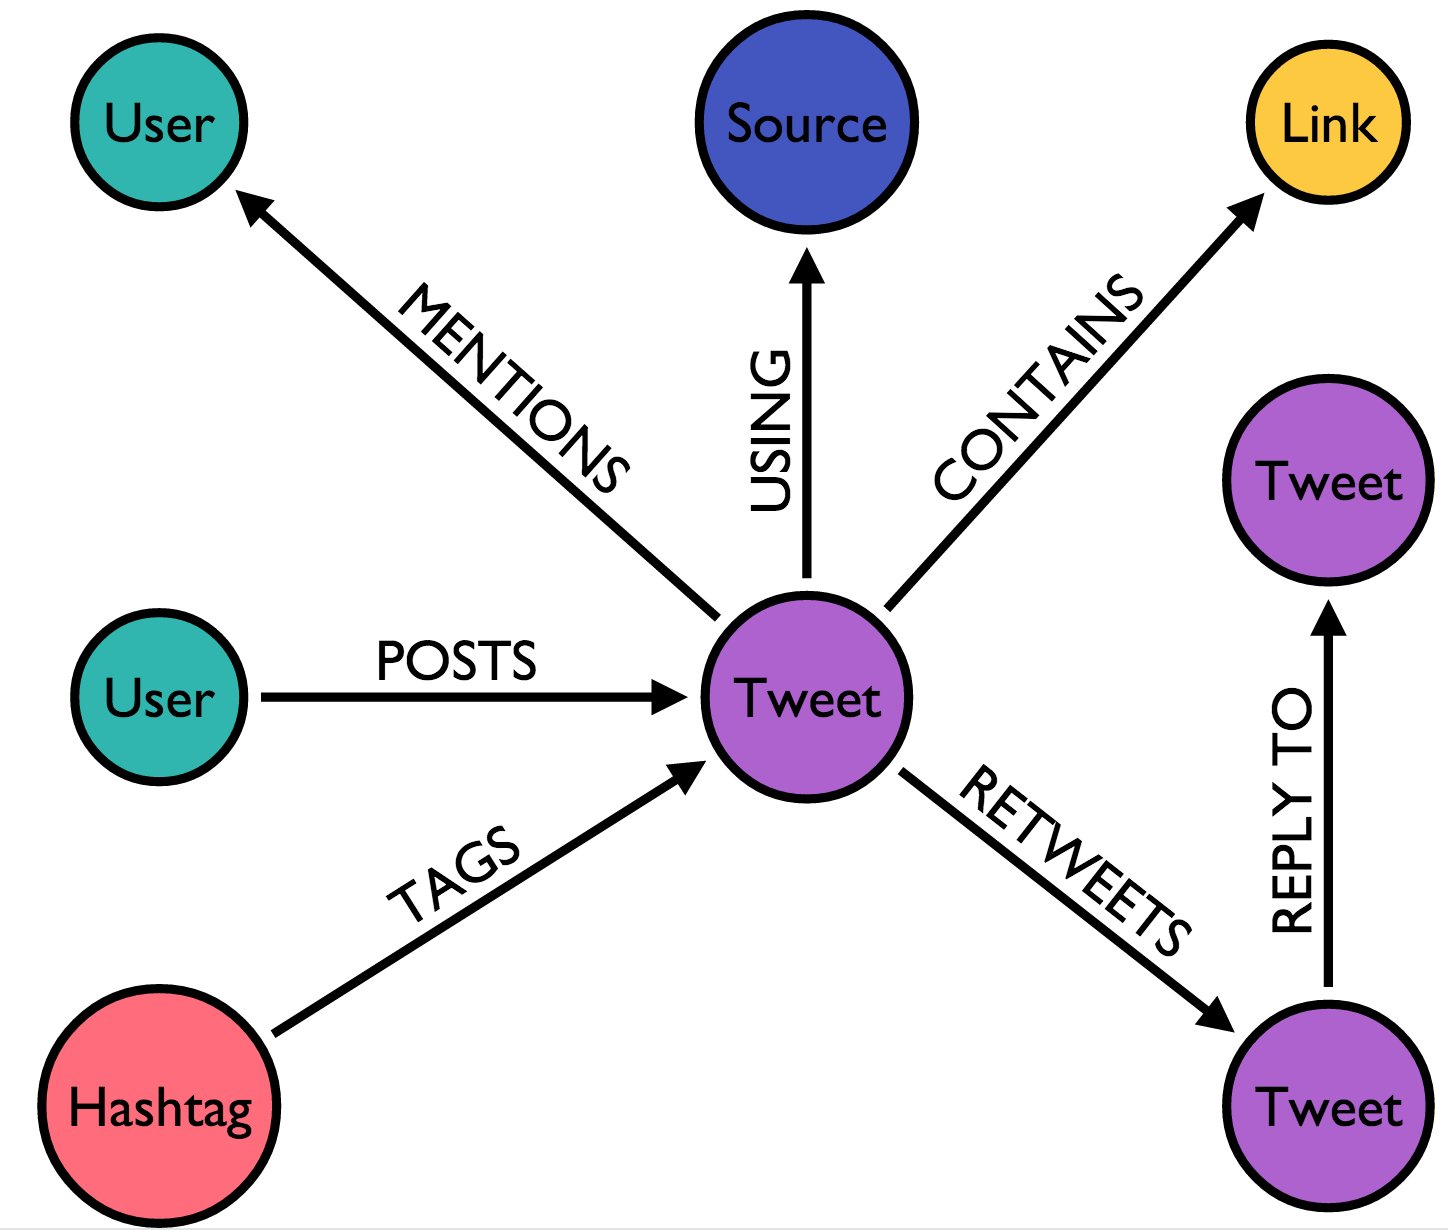
\includegraphics[width=0.5\linewidth]{images/graphdb_twitter}\caption{Example tweet data relationship}\label{fig:twitter}\end{center}\end{figure} Figure \ref{fig:twitter} illustrates the nodes involved in a standard tweet and the relationship link between them. The labeled nodes indicate the various operations which are involved in one the tweet. One interpretation of the figure \ref{fig:twitter} example is that a user posts a tweet, using the Twitter App which mentions another user and includes a hashtag and link.

\subsection{Relational Database}
A relational database (RDB) is a collection of data items organised as a set of tables, records and columns from which data can be accessed or reassembled in many different ways \cite{rdb}. The connected tables are known as relations and contain one or more columns which comprise of data records called rows. Relations can also be instantiated between the data rows to form functional dependencies.

\begin{itemize}
\item One to One: One table record relates to another record in another table.
\item One to Many: One table record relates to many records in another table.
\item Many to One: More than one table record relates to another table record.
\item Many to Many: More than one table record relates to more than one record in another table.
\end{itemize}


\subsection{Column-Orientated Database}
A column-orientated database (CODB) is a database management system that stores data tables as columns of data rather than as rows of data. The main objective of a CODB is to write and read data from the hard disk efficiently in an attempt to speed up querying time. A CODB has the ability to self index which uses less disk space than RDBMS which holds the same data. A CODB can also be highly compressed, resulting in aggregate functions such as MIN, MAX and SUM to be performed at a extremely high rate. \cite{cd}.

\begin{figure}[h]\begin{center}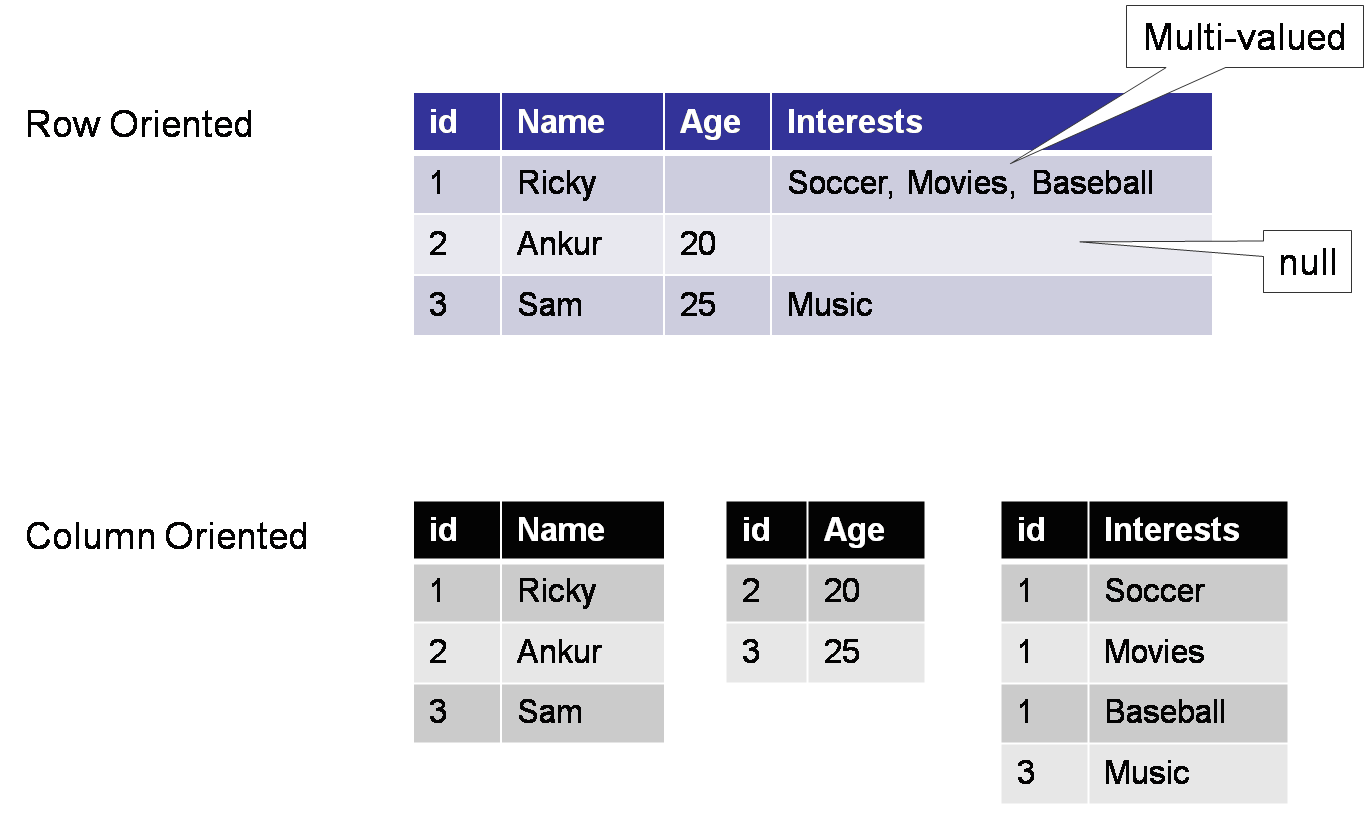
\includegraphics[width=1\linewidth]{images/codb}\caption{Column orientated database example}\label{fig:cod}\end{center}\end{figure}

Figure \ref{fig:cod} illustrates the comparison of a RDB model against a CODB model. Within the row based model the data contains both multiple values per record and null values. However in the CODB model null values are not required as each record contains a minimum and maximum of one value.

\section{Technology Evaluation}\label{techeval}
The technologies being evaluated in this project are outlined below.

\subsection{MongoDB}\label{mongo}
MongoDB is an open source cross-platform DODB. The premise for using MongoDB is simplicity, speed and scalability  \cite{md}. Its ever growing popularity, specifically amongst programmers, stems from the unrestrictive and flexible DODB data model which gives you the ability to query on all fields and boasts instinctive mapping of objects in modern programming languages. \cite{md} The database design of MongoDB is based on the JSON file format named BSON. 

A record in MongoDB is known as a document; a data structure composed of field and value pairs. The values of fields can include other documents, arrays and arrays of other documents. The key features of using MongoDB are its high performance data persistence, provide high availability and automatic scaling  \cite{md}.

\subsection{Neo4j}\label{neo}
Neo4j is an open-source NoSQL GODB which imposes the Property Graph Model throughout its implementation. The team behind the development of Neo4j describe it as an ``An intuitive approach to data problems" \cite{ndweb}. One of the reasons in which Neo4j is favoured predominantly amongst database administrators and developers is its efficiency and high scalability. This is in part due to its compact storage and memory caching for the graphs. ``Neo4j scales up and out, supporting tens of billions of nodes and relationships, and hundreds of thousands of ACID transactions per second." \cite{ndweb}

The key features of Neo4j which lends itself to users, developers and database administrators are its ability to establish relationships on creating, the equality of relationships permits the addition of new relationships being created after initial implementation at no performance cost and its use of memory caching for graphs which allows efficient scaling.

\subsection{Apache Cassandra}\label{cassandra}
Apache Cassandra is an open source column-orientated DDB that is designed for storing and managing vast amounts of data across multiple servers. ``Apache Cassandra is a highly scalable, high-performance distributed database designed to handle large amounts of data across many commodity servers, providing high availability with no single point of failure." \cite{cassandra}. Apache Cassandra define the key features of their database management system as ``continuous availability, linear scale performance, operational simplicity and easy data distribution across multiple data centres and cloud availability zones." \cite{cassandra}.  Figure \ref{fig:cass} illustrates an example record stored in a Cassandra database. \begin{figure}[h]\begin{center}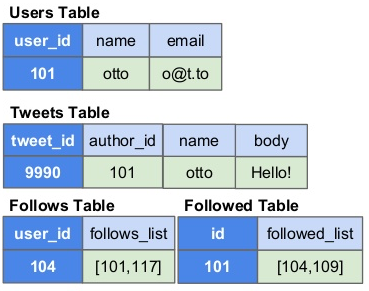
\includegraphics[width=0.70\linewidth]{images/cassandramodel}\caption{Example Cassandra record}\label{fig:cass}\end{center}\end{figure}

\subsection{MySQL}\label{mysql}
MySQL is a freely available open source RDB that uses Structured Query Language (SQL). MySQL is commonly used for web applications with its speed and reliability being a key feature. The MySQL database stores data in tables - a collection of related data - which consists of columns and rows. MySQL runs as a server and allows multiple users to manage and create numerous databases. 

SQL is a programming language used to communicate with databases through queries. SQL queries are used to perform tasks such as update or retrieve data in a database. The queries are in the form of command line language which include keyword statements such as select, insert and update.